\documentclass[../main.tex]{subfiles}


\begin{document}

In this chapter we will present our compression RNNs(C-RNN) designed to perform virtual sensing and provide reliable uncertainty estimates for its predictions. Recal we want to design virtual sensors  

Our general strategy is to use Recurrent Neural Networks(RNN) for modelling and prediction over time series data. 
The aleatoric uncertainty is modeled it as part of the phenomenon i.e. we learn to predict it from the data.
In terms of epistemic uncertainty, we focus on uncertainty stemming from OOD inputs, as we found in practice that it presents to biggest challenge for our applications. Our general strategy will be to model the training distribution $P(x)$, in order to be able to determine the likelihood of the input. That likelihood can then be used to estimate the epistemic uncertainty, or at least the component of it stemming from OOD inputs. Our models can be extended to account for parameter uncertainty by using techniques such as Monte-Carlo dropout\citep{gal2016dropout}. 

In the following subsections, we will begin by discussing how to model the training distribution, how to use that model to estimate epistemic uncertainty. Then we will present our full model, and how we train it.

\section{Modelling the training distribution}
\label{sec:information}

% Our approach to modelling the training distribution \pdf[train]{x} will be similar to variational autoencoders(VAE)~\citep{kingma2013auto}, adapted to sequential modelling. The only important difference is that the latent state for our model is deterministic. The main reason we use a deterministic latent state is speed. In typical deep learning 
Following the minimum description length principle\citep{rissanen1978modeling}, we model the data distribution by finding the model which compresses the data best. The link between data compression and distribution modelling is captured by the KL-divergence. Let \pdf{x|\theta} be a parameterized family of distributions, and \pdf[train]{x} be the distribution we wish to model. The KL-divergence
\begin{equation}
    \label{eq:kl}
    KL(P(x) || P(x|\theta)) = \int {\pdf[train]{x} log(\frac{\pdf[train]{x}}{\pdf{x|\theta}})} dx
\end{equation}{}
is equal to the expected number of additional bits required to compress the data from $P[train](x)$ using $P(x|\theta)$~\citep[chapter~5]{mackay2003information}. The KL hits its minimum of zero when the two distributions match exactly. Thus optimizing $\theta$ to minimize the number of bits required to compress the data is equivalent to minimizing the KL divergence between our family of distributions and the true distribution. 

Thus the task of modelling the distribution boils down to minimizing the expected number of bits required to compress data drawn from that distribution. We will use the training samples $X={x_1 \cdots x_n}$ to compute and optimize a monte-carlo estimate of that expectation. The KL becomes 
\begin{equation}
    \label{eq:mc_kl}
    KL(P(x) || P(x|\theta)) = -\sum_{x \in X} log{(\pdf{x|\theta})} dx
\end{equation}{}

Thus we simply need to minimize the negative log likelihood of the training data, under our distribution. 


Suppose we are compressing points drawn from a distribution $Q(x)$, the ideal lossless compressor for this distribution, denoted here as $C_Q(x)$, takes any input $x$ and outputs a compressed $z$ where the length of $z$ is equal to the negative log probability of $x$
\begin{equation}
    \label{eq:compression}
    len(z) = -log(Q(x))   
\end{equation}{}
Conversely, a probability model $Q(x)$ which assigns a probability $q$ to some point $x$, can be interpreted as assigning the input a compressed length of $-log(q)$. In short a probability distribution defines an ideal compressor and a compressor defines an ideal probability distribution. Note that this hold for lossless compression only, not lossy compression.  

Let $C(x|\theta)$ represent a family of compressors parameterized by $\theta$. We have already established that a compressor can also be interpreted as a probability distribution over the input space, let $P(x|\theta)$ represent the distributions. The KL-divergence between $P(x|\theta)$ and the true data distribution $P(x)$
\begin{equation}
    KL(P(x) || P(x|\theta)) = \sum_{x \in X}{P(x) log(\frac{P(x)}{P(x|\theta)})}
\end{equation}{}
is equal to the expected number of additional bits required to compress the data from $P(x)$ using $P(x|\theta)$~\citep[chapter~5]{mackay2003information}. The KL hits its minimum of zero when the two distributions match exactly. Thus optimizing $\theta$ to minimize the number of bits required to compress the data is equivalent to minimizing the KL divergence between our family of distributions and the true distribution. 

% To have lossless compression, we need to account for the number of bits required to recover $x$ from the compressed code $z$ perfectly. 

To learn compression models from data, we can train Autoencoders(AEs) which learn to compress inputs $x$ to compressed codes $z$ then reconstruct $x$. 
The number of bits an AE needs to compress an input has two components, the number of bits in the compressed code, and the number of bits it takes to go from the model's reconstruction to the original input, since we require perfect reconstruction for this scheme to be sound.
Those are commonly referred to as the likelihood and reconstruction loss respectively in the context of autoencoders. It is important to account for both, since it is trivial to compress data into short codes if we don't need to reconstruct it, and it is trivial to perfectly reconstruct data if we don't need to compress it.

To optimize $\theta$ we do not need to actually generate the compressed codes and see how long they are, instead we can resort to probabilistic modeling again via \cref{eq:compression}. 
For the compressed codes, we can define some prior probability distribution in some latent space, and let the model output a code in that space. The length of the code is then determined by the probability the prior assigns it again via \cref{eq:compression}, we call this $c_{l}(x)$. For the reconstruction error, instead of having the model output an exact reconstruction, we let the model output a probability distribution over the input space x, then the length of the code needed to specify the input exactly is also determined by the probability of the input under this distribution also via \cref{eq:compression}, we call this $c_{r}(x)$.

To sum up the length of the compressed code word under for an input 
\begin{equation}
    \label{eq:compression_cost}
    c(x) = c_{l}(x) + c_{r}(x)
\end{equation}{}

and the implied probability of the input is then $P(x|\theta) = 2^{-log(c(x))}$. 

% \section{From probabilities to uncertainties}

% Once we have a model for the training distribution, the question becomes how to use that model to estimate the epistemic uncertainty for our prediction.
% Assume we have found parameters $\theta$ which define our final model. To be clear $\theta$ defines a model which both predicts $y$ from $x$ and estimates the training distribution density i.e. gives us an estimate of \pdf[t]{x} where \dist{t} is the training distribution. 
% For clarity in this section, we assume without loss of generality that $\theta$ is a point estimate rather than a whole posterior over parameters. 

% For inputs from the training distribution we simply use $\theta$ to make predictions. Our problem lies in the fact that we might encounter inputs which did not come from the training distribution. This means that for some inputs, our model is not \emph{valid}. The question is how to account for this uncertainty. 

% We let \dist{t} be the training distribution, \dist{u} be the universal distribution from which inputs come at test time. We further break down the universal distribution as a mixture of the training distribution and another distribution \dist{o} so that
% \begin{equation}
%     \pdf[u]{x} = \pi_\dist{t} \, \pdf[t]{x} + \pi_\dist{o} \, \pdf[o]{x}
% \end{equation}{}
% where $\pi$ represents the mixture parameters which are positive and sum to one. So that \dist{o} captures the regions of \dist{u} which \dist{t} does not cover. 

% Given this model, we can reason about the probability that an observed point $x$ came from the training distribution
% \begin{equation}
%     \label{eq:dataset_posterior}
%     \pdf{t|x} = \frac{\pdf[t]{x} \, \pi_\dist{t}}{\pdf[u]{x}}
% \end{equation}{}
% % and $\pdf{x} = \pdf[t]{x} \, \pi_\dist{t} + \pdf[o]{x} \, \pi_\dist{o}$.

% $\pdf[t]{x}$ is estimated by our model. The remaining terms in \cref{eq:dataset_posterior} have to be treated as hyper-parameters or priors. 
% With this our final prediction should be 

% \begin{equation}{}
%     \pdf{y|x} = \pdf{t|x} \, \pdf{y|x, \theta} + \pdf{o|x} \, \pdf{y|x, \alpha}
% \end{equation}

% Where \pdf{y|x, \alpha} is a predictive model for \pdf{y|x} on the regions not covered by the training distribution, parameterized by $\alpha$. Strictly speaking $\alpha$ is unknown to us. As alluded to in the closing discussion of \cref{ch:background}. The reason should now be clearer, \pdf{y|x, \alpha} is a model for data which we have not seen. Of course, in the presence of prior knowledge, we can suppose some reasonable model for \pdf{y|x, \alpha}. 
% For example, with classification models there is an easy solution, let \pdf{y|x, \alpha} simply predict the uniform distribution over all the classes. This way it will act as a smoother for the classifier, and as we move further away from the data distribution, the predictions get more uniform.

% For regression, suppose our model \pdf{y|x, \alpha} outputs a mean and std $\mu_\alpha$ and $\sigma_\alpha$ of a Gaussian. We may, for example, simply define the model to output a unit Gaussian s.t. \pdf{y|, x, \alpha} = $\mathcal{N}(y; 0, 1)$. We could also use richer prior knowledge. Let $\pdf{y|x, \theta} = \mathcal{N}(y; \mu_y, \sigma_y)$. We can then define $\pdf{y|x, \alpha} = \mathcal{N}(y; \mu_y, \sigma_\alpha)$, with $\sigma_\alpha$ being a hyper-parameter. This model predicts that the mean prediction remains the same, but the std should go higher to account for the higher uncertainty. 
% % There are in fact models which use this formulation, noise contrastive priors~\citep{Hafner2018NoiseCP}.
% Thus, in order to make sound predictions in the strictly non i.i.d regime we described, certain prior assumptions must be made.

% In the absence of enough knowledge to define those priors, the shortcut taken is to simply use our estimate of \pdf[t]{x} as an uncertainty score. If it is high enough, we use the prediction from our model, if it is below a certain threshold, we simply signal that a prediction cannot be made. 

% \ahmed{This subsection will be developed later. Possibly moved to background}


\section{Compression RNNs(C-RNN)}
\label{sec:model}

\begin{figure}
    \centering
    \label{fig:architecture}
    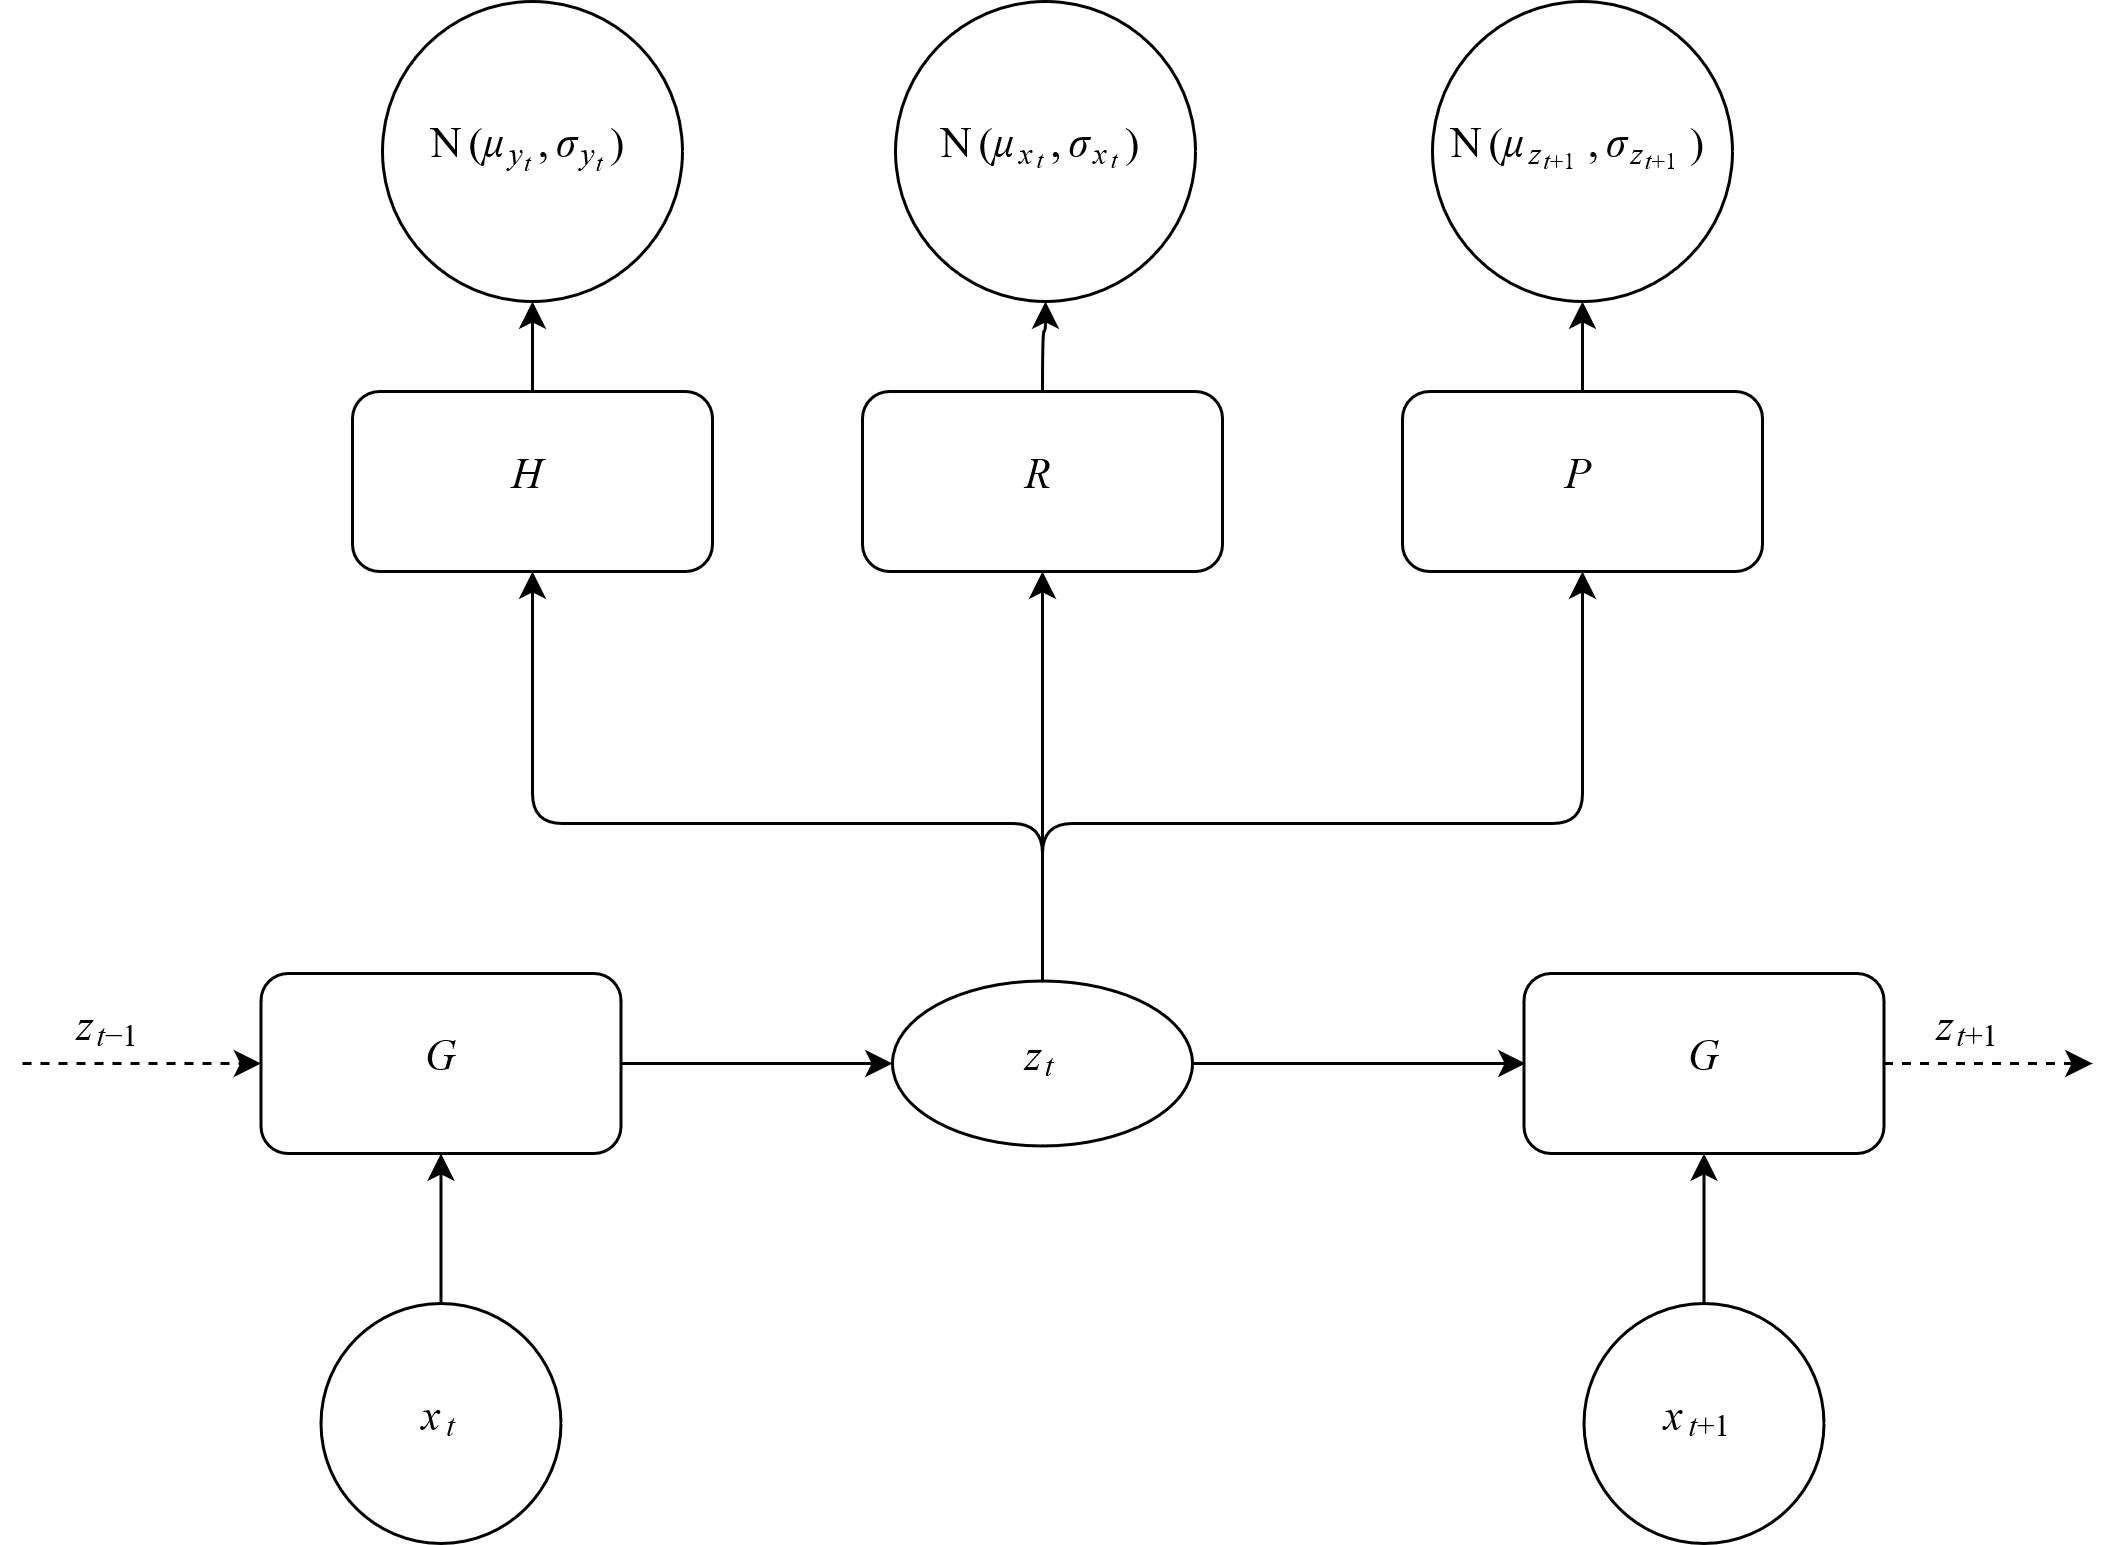
\includegraphics[width=\textwidth]{Approach/rnn_architecture.png}
    \caption{The RNN architecture, at each timestep the network outputs the mean and std of three Gaussians}
\end{figure}

\subsection{Model}

In this section we will introduce our recurrent models which act as both the predictor for $y$ and density estimator for \pdf[t]{x}. 
The architecture is depicted in \cref{fig:architecture}, The model is made up of four parameterized functions, all neural networks. Let $x_t$ denote our input at time t, $z_t$ our latent states, and $y_t$ our targets and $\theta$ our model parameters.
\begin{enumerate}
    % \item $f(x)$ is the projection network, which maps the inputs $x_t$ into the representation fed to the recurrence.
    \item $g(x, z)$ is the recurrent module, which takes $z_{t-1}$ and $x_t$ to predict $z_t$
    \item $h(z)$ is the prediction module, which takes $z_t$ and predicts $y_t$
    \item $r(z)$ is the reconstruction module, which takes $z_t$ and predicts $x_t$
    \item $p(z)$ is the prior module, which takes $z_{t-1}$ and predicts $z_t$
\end{enumerate}

The prediction, prior and reconstruction modules are our model outputs, for each time-step each module parameterizes a Gaussian via outputting a mean and standard deviation(std). 
The prediction module $h(.)$ models $P(y_t|x_t)$. The prior module gives the prior models $P(z_{t+1}| z_t)$. The reconstruction module gives $P(x_t|z_t)$. 

As discussed in \cref{sec:information}, the prior is used to define a distribution in latent space, which in turn allows us to compute the length of the compressed code for $z$. Concretely $P(z_t) = \mathcal{N}(z_t; \mu_{z_t}, \sigma_{z_t})$ where $\mu_{z_t}, \sigma_{z_t} = p(z_{t-1})$. Then $c_l(z_t) = -log(P(z_t))$. 
Analogously the reconstruction module gives a probability over the input space which then allows to compute the length of the code to specify $x$. Adding them together give the total compression cost for an input as per \cref{eq:compression_cost}, from this we can recover the probability our model assigns to an input via \cref{eq:compression}.

\subsubsection{Uncertainty breakdown}

Our model expresses uncertainty via two outputs. The aleatoric uncertainty is expressed in the std of the predictive distribution, that is $\sigma_y$.

Our model expresses epistemic uncertainty via the compression cost of the input. That is 
\ahmed{TODO}


\subsection{Training}

Our loss function is composed of the prediction loss, reconstruction loss, and the latent loss.
The overall loss for training our model is 
\begin{equation}
    \label{eq:overall_loss}
    \mathcal{L} = \mathcal{L}_{y} + \lambda (\mathcal{L}_{x} + \mathcal{L}_{z})
\end{equation}{}
All three are components are formulated as Negative Log-Likelihoods(NLL)
$$
    \mathcal{L}_{y} = -\log (\mathcal{N}(y; \; \mu_y, \sigma_y))
$$
where $\mu_y$ and $\sigma_y$ are the outputs of $h(.)$. Similarly, 
$$
    \mathcal{L}_{x} = -\log(\mathcal{N}(x; \; \mu_x, \sigma_x))
$$
where $\mu_x$ and $\sigma_x$ are the outputs of $r(.)$. and 
$$
    \mathcal{L}_{z} = -\log(\mathcal{N}(z; \; \mu_z, \sigma_z))
$$
where $\mu_z$ and $\sigma_z$ are the outputs of $p(.)$. All those losses factorize over the time. For example, the prediction loss for a sequence is

\begin{equation}
    % \label{eq:overall_loss}
    \mathcal{L}_{y} = \sum_{t=1}^{n} -\log (\mathcal{N}(y_t; \; \mu_{y_t}, \sigma_{y_t}))
\end{equation}{}

The model is trained with the Adam optimizer~\citep{kingma2014adam}, following a cosine learning schedule~\citep{loshchilov2016sgdr}. However, we have made two modifications to improve the training.

\subsubsection{KL annealing}

A known issue for variational autoencoders is KL-vanishing~\citep{bowman2015generating}, where early on in training the latent regularizer prevents the model from encoding information in the latent state, in order to push the latent loss down. We saw a similar problem in our setting, although our latent loss is an NLL loss. In our context it is also important to remember that we are not only autoencoding the inputs, but we are also making predictions. In fact the predictions are our main task. We found that when training the predictor and generative model as described, the predictive model is over-regularized and prediction quality goes down. Following~\citep{liu2019cyclical}, we use a cyclical annealing schedule for the compression loss. Specifically, our schedule is over $\lambda$ in \cref{eq:compression}. The $\lambda$ parameter starts a cycle at zero and increases linearly, reaching its maximum at the mid point of the cycle, then remains constant for the rest of the cycle. 

\subsubsection{Compression loss weighting}

Our motivation for modelling the density of the training is distribution is to use it to determine how reliable our prediction is for an input. Assuming our model performs well on points drawn from the training distribution.
If an input is likely under the training distribution, it would follow that our model is likely to give a good prediction for that input. The problem comes from that fact that our model may not be performing equally well over the whole training distribution. This may be due to bad priors, poor optimization, or simply the complexity of the behavior of $P(y|x)$ in certain regions. Due to such factors, there may be sparse regions where the model performs better, and dense regions where the model performs worse. In short, the density of the training distribution may not be perfectly correlated with the model's performance. In order to get higher quality uncertainty estimates we wish to place more mass in the input regions where the model performs well, and less in regions where the model performs poorly. 

In order to bias our density estimator to place less mass in regions where the model performs poorly, we use a weighted compression loss, where points with high prediction loss get less weight. Thus for a mini-batch during training the compression loss becomes 
\begin{equation}
    c(x) = \sum_{i=1}^{n} \sum_{t=1}^{m} w^i_t \; c(x^i_t)  
\end{equation}

Where the $w^i_t$ are weights assigned according to how well the predictive model performs on that point. The weight $w^i_t$ should be large when the model predicts $y^i_t$  well from $x^i_t$ and low otherwise. The intuition here is the same as for representation learning, where the best representation depends on the downstream task~\citep{hjelm2018learning}.

The weights should depend on our predictive errors $\mathrm{E}$. Let $\mathrm{E} = |Y - \hat{Y}|$ be a vector containing absolute error of between our model predictions and the targets for a training mini-batch. Let $W$ be the vector containing our weight, we can define $W$ with 
\begin{equation}
    W = Softmax(\mathrm{E} \cdot t)
\end{equation}{}

Where t is a temperature hyperparameter. If we set $t$ to zero, we can get back the original formulation, and as we increase the temperature we can bias the model towards placing more mass in regions where the error is small.

\textbf{Decoupling uncertainties} Our density estimator is used to obtain epistemic uncertainties. One issue with using the absolute error to obtain the weights, is that we would be conflating epistemic and aleatoric uncertainties. The error could be large simply because the aleatoric uncertainty is large, rather than the model performing poorly. Thus if the error is large, and the model's estimate of aleatoric uncertainty is proportionally large, we can at least consider the model well calibrated. The cases we really want to capture with epistemic uncertainty is when there is a mismatch between the model's error and its estimate of aleatoric uncertainty, particularly when the model is overconfident. One quantity which captures this is the absolute error measured in number of stds
\begin{equation}
    \mathrm{E_{std}} = \frac{|Y - \hat{Y}|}{\Sigma_y}
\end{equation}{}
 where $\Sigma$ is a vector containing the predicted stds($\sigma_y$) for each point. Thus we define the weights to be a softmax over $\mathrm{E_{std}}$ rather than $\mathrm{E}$. 
 
 
 \section{Discussion}
 



\end{document}
